%        File: 24.03.20.tex
%     Created: пн мар 23 10:00  2020 M
% Last Change: пн мар 23 10:00  2020 M
%
\documentclass[algebra,twocolumn]{pum}
\listnumber{3}
\date{24.03.20}
\classname{8-Д}
\lesson{практикум }
\pgfplotsset{school/.append style={axis lines=middle, xlabel={$x$}, ylabel={$y$}, axis equal, grid=both, xlabel style={at={(ticklabel* cs:1)}, anchor=north west}, ylabel style={at={(ticklabel* cs:1)}, anchor=north west}},graphic/.style={mark=none,thick=8pt,samples=100}}
\begin{document}

\subsubsection*{Задачи на построение графиков функций}
График функции можно строить одним из двух способов:
\begin{enumerate}[nosep]
  \item Заполнить таблицу с координатами точек, вычисленных по аргументу и соотвествующему значению функции, после чего последовательно соединить точки, проходясь по системы координат слева направо.
  \item Произвести преобразования графиков функций
    \begin{equation*}
      y=x,\quad y=\frac{1}{x},\quad y=x^2,
    \end{equation*}
    используя растяжения/сжатия, отражения и параллельный перенос.
\end{enumerate}
В следующих номерах необходимо воспользоваться вторым способом.

  \begin{exercises}
    \begin{question}
      Построить графики функций и назвать кривую, которую они собой представляют:
      \begin{multicols}{2}
        \begin{enumerate}[label=\arabic*)]
        \item $y=2x+3$ 
        \item $y=-\frac{3}{x-1}$ 
        \item $y=(x-3)^2$ 
        \item $y=3(x-2)+5$ 
        \item $y=\frac{5}{x+1}+1$ 
        \item $y=(2-x)^2+1$ 
        \item $y=-(x-2)-1$ 
        \item $y=\frac{x-2}{x+3}+5$ 
        \item $y=2(x+3)^2+1$ 
        \item $y=3(x+1)-2(x-2)$ 
        \item $y=\frac{x-2}{x^2-4}$ 
        \item $y=-x^2-2x$ 
      \end{enumerate}
    \end{multicols}
  \end{question}

  По графикам определить функцию и найти координаты точек пересечения графиков друг с другом и с осями координат. Сравнить полученные значения с точными значениями.
\begin{question}
  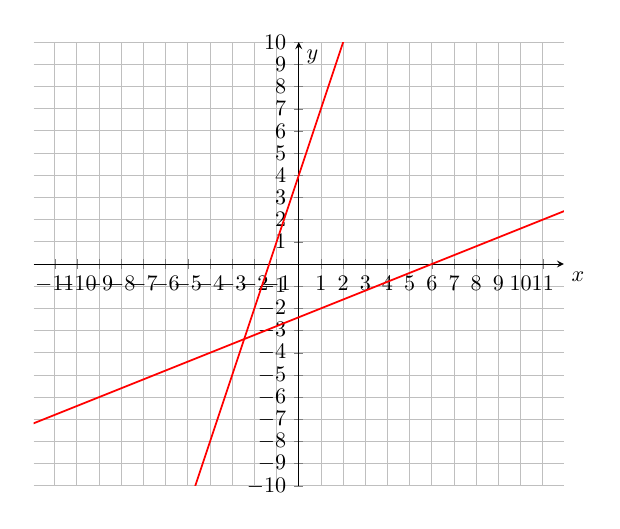
\begin{tikzpicture}[scale=0.8]
    \begin{axis}[
        school,
        width=10cm,
        xmin=-10, xmax=10,
        ymin=-10, ymax=10,
        xtick distance=1,
        ytick distance=1,
      ]
      \addplot[graphic,red,domain=-15:15] {0.4*(x-6)};
      \addplot[graphic,red,domain=-15:15] {3*x+4};
    \end{axis}
  \end{tikzpicture}
\end{question}
\begin{question}
  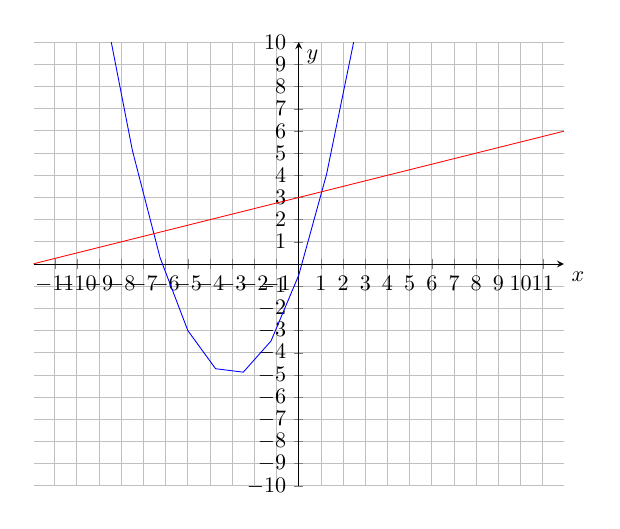
\begin{tikzpicture}[scale=0.8]
    \begin{axis}[
        school,
        width=10cm,
        xmin=-10, xmax=10,
        ymin=-10, ymax=10,
        xtick distance=1,
        ytick distance=1,
      ]
      \addplot[blue,domain=-15:15] {0.5*(x+3)^2-5};
      \addplot[red,domain=-15:15] {0.25*x+3};
    \end{axis}
  \end{tikzpicture}
\end{question}
\begin{question}
  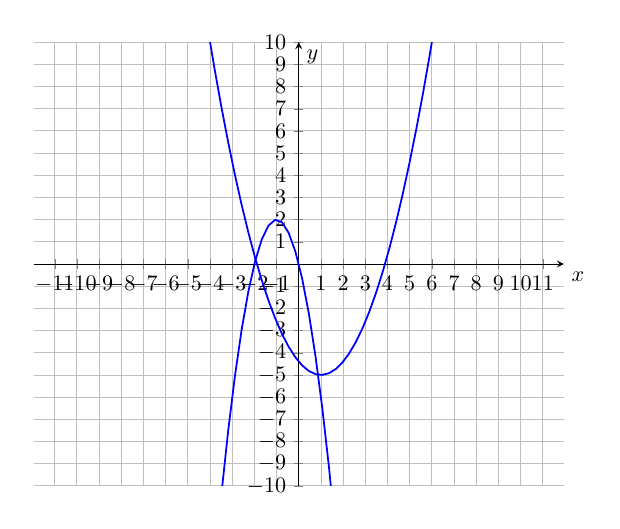
\begin{tikzpicture}[scale=0.8]
    \begin{axis}[
        width=10cm,
        xmin=-10, xmax=10,
        ymin=-10, ymax=10,
        axis lines=middle,
        axis equal,
        grid=both,
        xtick distance=1,
        ytick distance=1,
        xlabel=$x$,
        ylabel=$y$,
        xlabel style={at={(ticklabel* cs:1)}, anchor=north west},
        ylabel style={at={(ticklabel* cs:1)}, anchor=north west}
      ]
      \addplot[blue,mark=none,domain=-15:15,thick=8pt,samples=100] {-2*(x+1)^2+2};
    \addplot[blue,mark=none,domain=-15:15,thick=8pt,samples=100] {0.6*(x-1)^2-5};
    \end{axis}
  \end{tikzpicture}
\end{question}
\begin{question}
  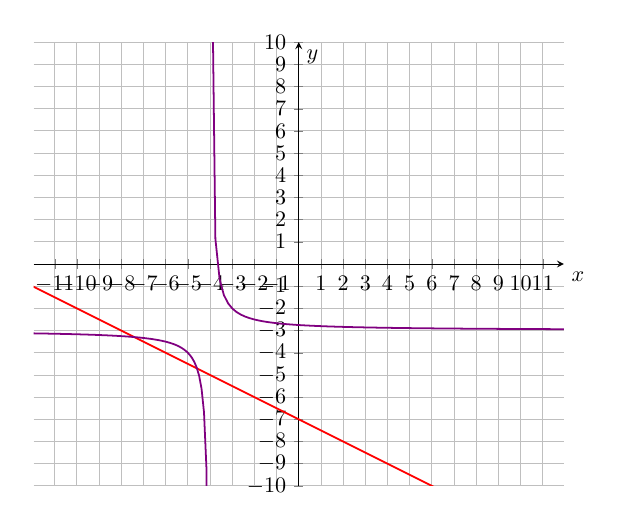
\begin{tikzpicture}[scale=0.8]
    \begin{axis}[
        width=10cm,
        xmin=-10, xmax=10,
        ymin=-10, ymax=10,
        axis lines=middle,
        axis equal,
        grid=both,
        xtick distance=1,
        ytick distance=1,
        xlabel=$x$,
        ylabel=$y$,
        xlabel style={at={(ticklabel* cs:1)}, anchor=north west},
        ylabel style={at={(ticklabel* cs:1)}, anchor=north west}
      ]
      \addplot[red,mark=none,domain=-15:15,thick=8pt,samples=100] {-x/2-7};
      \addplot[violet,mark=none,domain=-15:-4.05,thick=8pt,samples=100] {1/(x+4)-3};
      \addplot[violet,mark=none,domain=-3.95:15,thick=8pt,samples=100] {1/(x+4)-3};
    \end{axis}
  \end{tikzpicture}
\end{question}
\begin{question}
  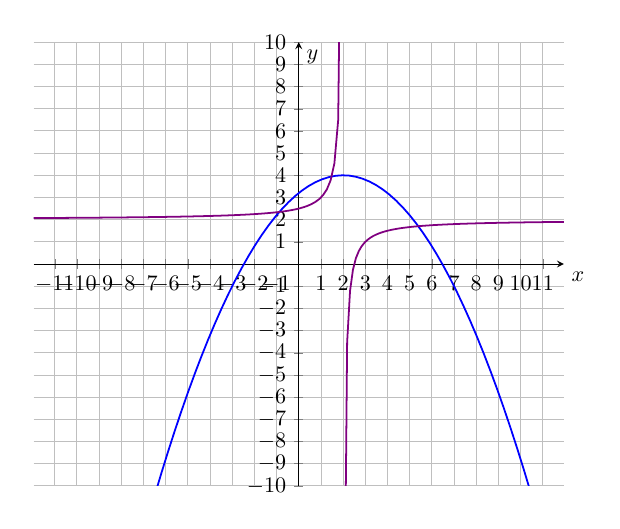
\begin{tikzpicture}[scale=0.8]
    \begin{axis}[
        width=10cm,
        xmin=-10, xmax=10,
        ymin=-10, ymax=10,
        axis lines=middle,
        axis equal,
        grid=both,
        xtick distance=1,
        ytick distance=1,
        xlabel=$x$,
        ylabel=$y$,
        xlabel style={at={(ticklabel* cs:1)}, anchor=north west},
        ylabel style={at={(ticklabel* cs:1)}, anchor=north west}
      ]
      \addplot[blue,mark=none,domain=-15:15,thick=8pt,samples=100] {-0.2*(x-2)^2+4};
    \addplot[violet,mark=none,domain=-15:1.95,thick=8pt,samples=100] {-1/(x-2)+2};
    \addplot[violet,mark=none,domain=2.05:15,thick=8pt,samples=100] {-1/(x-2)+2};
    \end{axis}
  \end{tikzpicture}
\end{question}
\begin{question}
  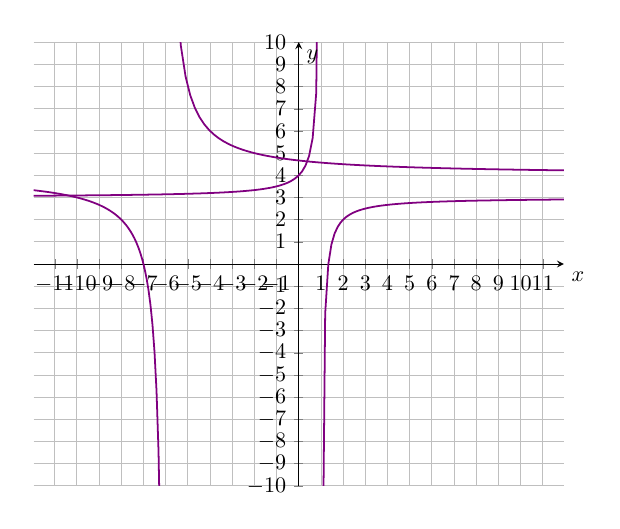
\begin{tikzpicture}[scale=0.8]
    \begin{axis}[
        width=10cm,
        xmin=-10, xmax=10,
        ymin=-10, ymax=10,
        axis lines=middle,
        axis equal,
        grid=both,
        xtick distance=1,
        ytick distance=1,
        xlabel=$x$,
        ylabel=$y$,
        xlabel style={at={(ticklabel* cs:1)}, anchor=north west},
        ylabel style={at={(ticklabel* cs:1)}, anchor=north west}
      ]
      \addplot[violet,mark=none,domain=-15:-6.05,thick=8pt,samples=100] {4/(x+6)+4};
      \addplot[violet,mark=none,domain=-5.95:15,thick=8pt,samples=100] {4/(x+6)+4};
      \addplot[violet,mark=none,domain=-15:0.95,thick=8pt,samples=100] {-1/(x-1)+3};
    \addplot[violet,mark=none,domain=1.05:15,thick=8pt,samples=100] {-1/(x-1)+3};
    \end{axis}
  \end{tikzpicture}
\end{question}
\end{exercises}

\end{document}


